\documentclass{article}
\usepackage[margin=1in]{geometry}
\usepackage{graphicx}
\usepackage{amsmath}
\usepackage{multirow}
\usepackage{multicol}
\usepackage{wrapfig}



%\topmargin 0pt
%\oddsidemargin 12pt
%\evensidemargin 12pt
\interfootnotelinepenalty=10000


\begin{document}
\title{Uncertainty in Local Sequence Alignment}
\author{Yi Tian Xu\\260520039}

\maketitle

\abstract{We generalized Basic Local Alignment Search Tool  reference sequence with uncertainty information. }

%\begin{multicols}{2}

\section{Introduction}

Basic Local Alignment Search Tool (BLAST) has become famous in bioinformatics for its capability in comparing a query sequence with a database of sequences. However, BLAST does not handle the case when the reference sequence contains probabilistic information. More specifically, we may not know with total certainty the exact base at certain position of the sequence. Such case may occur from the ambiguity at certain positions in the sequence data induced by experimental error. For example, state of the art DNA sequencers, such as Roche/454, Illumina and SOLiD, have an error rate between 0.1\% to 1\% that varies according to the read length. \cite{sequencers} This error can be modelled as a confidence score for each nucleotide according to its position in the reads. Another scenario where probabilistic information can be added to sequence data is ancestral sequence reconstruction. Such sequence, derived with seldom known true phylogeny, uncertainty in observational data and the assumption of maximal parsimony \cite{parsimony}, can also be expressed with a confidence score at each nucleotide. 

BLAST maximizes a similarity measure between sequences to search for an alignment. This similarity measure assign a score for insertion, deletion and substitution base of the rarity of mutation. \cite{blast} For example, considering that transversions are less likely than transitions, a DNA sequence ``AAA" may have a higher similarity score when aligned to ``AAG" than ``AAT". Nevertheless, when we add information on the uncertainty of the sequence, we may expect a different bahaviour; if the last nucleotide in the sequence ``AAT" had much less confidence than the last nucleotide in ``AAG", we may want the alignment with ``AAT" to have a higher similarity score than with ``AAG". This behaviour must be incorporated in two phases of BLAST: (1) the database indexing phase and (2) the hit expansion phase.  

An local alignment search tool that utilizes probabilistic information in the reference sequence data not only allow us to find better alignments, but also contributes to the quality of our analysis in the subsequence steps of our research pipeline. To answer to this need, we generalize BLAST by modifying the similarity measure and by developing a new method for indexing the database. We test our method on a DNA sequence data; a portion of CHR22, a predicted BoreoEutherian ancestor sequence, of 604,466 nucleotides was used as our reference sequence. Each nucleotide in the sequence has an associated confidence value on the correctness of the prediction. We assume that each position in the sequence has equal chance of being one of the other three nucleotides if it were predicted wrong. 

\section{Method}

BLAST runs in three steps: (1) it preprocesses the reference sequence by constructing a database of high scoring words mapped to their position on the sequence, (2) upon input of a query sequence, it splits this sequence into words and for each subsequence, it searches for a match in the database, and finally (3) for each match, it extends the alignment using sequence alignment and select the alignment(s) with the highest score. \cite{blast} To include uncertainty information in this process, we modify the similarity measure in the local sequence alignment algorithm and develop conditions to find high scoring words. 

\subsection{Similarity measure}

Classical sequence alignment is based on a dynamic programming that computes some similarity measure for each pair of nucleotides of the input sequences. \cite{blast} The similarity measure generally scores according to the likeness of the substitution, insertion and deletion. In our method, we use $m = 2$ for identity, $s_t = -1$ for transition and $s_v = -2$ for transversion substitutions. For simplicity, we only consider linear gap function, $g(x)=-2x$. This measuring system can be formalized in the following way. Let $M$ be the substitution matrix. 
\begin{equation}
	M = \begin{bmatrix}
		m & s_v & s_t & s_v\\
		s_v & m & s_v & s_t\\
		s_t & s_v & m & s_v\\
		s_v & s_t & s_v & m\\
	\end{bmatrix}
\end{equation}
Given the alphabet $\Sigma =$ \{A,C,G,C\}, we can represent a nucleotide $a \in \Sigma$ as a vector $\vec{u}_a = (u_{\mbox{A}}, u_{\mbox{C}}, u_{\mbox{G}}, u_{\mbox{T}})$ where each entry $u_x = 1$ if $x = a$ or 0 otherwise. Thus, the score for matching two nucleotides, $a$ and $b$ can be formulate as $s(a,b) = \vec{u}_aM\vec{u}_b$.

To include the uncertainty information of the sequence, we use the expected similarity score. That is, given the reference nucleotide $a$ and its confidence probability $p$, we construct the vector $\vec{u}_{a,p} = (u_{\mbox{A}}, u_{\mbox{C}}, u_{\mbox{G}}, u_{\mbox{T}})$ where each entry $u_x = p$ if $x=a$ or $(1-p)/3$ otherwise. The score for matching a query nucleotide $b$ is $s(a,b,p) = \vec{u}_{a,p}M\vec{u}_b$. We can see that when there is no uncertainty, $p=1$, $u_{a,p} = u_a$ for all $a \in \Sigma$, and it involves no change in complexity of the local alignment algorithm. 

For the chosen parameters $m, s_t$ and $s_v$ as described previously, Figure \ref{figure:score_graphs} shows the substitution score according to the variation in the confidence $p$. We can see that, this scoring system penalize less for mismatches and rewards less for matches in the presence of uncertainty. It also allow a transversion to score higher than a transition when the confidence for the nucleotide at the transversion substitution is more than 0.6 less than the confidence at the transition substitution. It also allow a mismatch to score higher than a match when the confidence value is lower enough. Finally, it allows a transversion to more rewarding than a gap in the presence of uncertainty. 

\begin{figure}[tbp]
\begin{center}
\caption{Substitution score variation according to the confidence value. When the confidence value is 1.00, the match, transition and transversion score reflect the case when the reference sequence has no uncertainty.}
   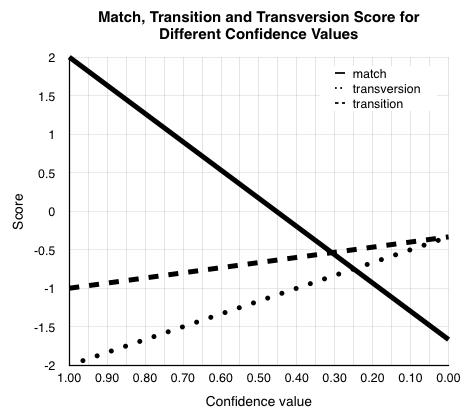
\includegraphics[width=0.50\textwidth]{score_graph}
\label{figure:score_graphs}
\end{center}
\end{figure}

\subsection{Database Indexing}

Classical sequence alignment algorithms (such as Smith-Waterman) are unfeasible for aligning long sequence of millions of nucleotides. Hence, the heuristic algorithm, BLAST, is developed. \cite{blast} This method preprocesses the reference sequence $G$ by compiling a list of high-scoring $w$-mers. One can construct a hashtable keyed by all substrings of length $w$ in $G$ and valued by a list of the $w$-mers' occurred locations in $G$. Thus, the local alignment of a query sequence $q$ can be estimated at the locations in $G$ given by its $w$-mers that match the $w$-mers in $q$. When a match, or hit, $h$ such that $q = q_1hq_2$ is found in the hashtable, BLAST subsequently perform the alignment of the prefix $q_1$ and suffix $q_2$ to obtain a complete alignment and score. The alignment with the highest score is then returned as best alignment.

In the context of uncertainty, we constructs the $w$-mers by treating all positions in the reference sequence with less than a certain confidence threshold, $\delta_p$, as a wildcard character. For example, for $w = 3$, a reference substring ``AAA" with confidences 1.00, 0.97 and 0.91 respectively expands to a set of 4 trimers, \{``AAA", ``AAC", ``AAG", ``AAT"\}, if $0.91 < \delta_p \leq 0.97$ or 16 trimers, \{``AAA", ``ACA", ``ACC", ..., ``ATT"\}, if $\delta_p > 0.97$. 

This hashtable construction has two main issues. First, the running time for performing this construction has exponential worst case $O(4^wLw)$ where $L$ is the length of $G$. Depending on the distribution of the confidences, the method can be extremely inefficient for high $\delta_p$. In the case of our reference sequence, CHR22, Figure \ref{figure:conf_cum} shows the cumulative distribution of its confidence values. First, we notice that there is no confidence values lower than 0.39, . Second, we observe a non-uniform distribution of the confidence values. In particular, around 80\% of the values are above 0.9, suggesting that a high confidence filtering threshold can be beneficial to the time efficiency of the method. More precisely, if the the proportion of nucleotides with confidence value less than a chosen $\delta_p$ is $f$, then the expected number of nucleotides in a $w$-mer that need to be expanded is $fw$. Thus, assuming independence between w-mers and nucleotides, the worst case running time is $O(4^{fw}Lw)$. For example, we can choose $\delta_p$ such that $f = 1/w$ and the time complexity becomes polynomial, i.e.: $O(Lw)$. 

The second issue is that low-scoring $w$-mers can be introduced to the database when we have uncertainty at multiple consecutive positions. For example, the expansion of a trimer ``AAA" with confidence values 0.5 for every nucleotide contains ``CCC", but the similarity score between the two is -3.5. It can be unclear where the line of separation between low and high-scoring $w$-mers should be defined. Figure \ref{figure:score_dist} shows the observed distribution of scores for matching sequences of lengths 3 and 7. We observe that a large portion of their weights tilt to the negative region, suggesting that a high-scoring $w$-mer may not necessarily need to be close to the score of a complete match (6 for trimers and 14 for 7-mers). Acknowledging the distribution, we attempt to investigate more on this issue experimentally by setting up a score threshold, $\delta_s$, which filters hits with scores less than $\delta_s$.

\begin{figure}[tbp]
\begin{center}
\caption{Cumulative distribution of the confidence value in the entire reference sequence (on the left) and in the first 1000 nucleotides of the reference sequence (on the right).}
   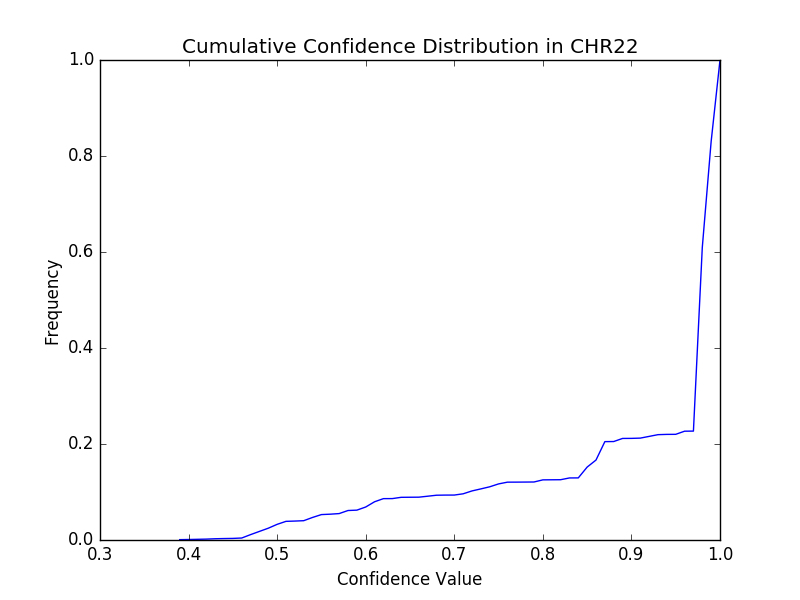
\includegraphics[width=0.49\textwidth]{conf-cum}
   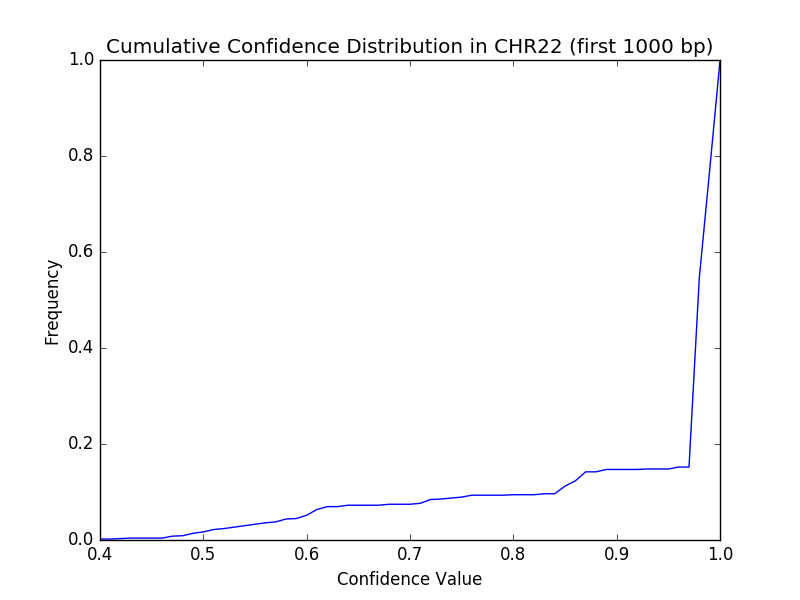
\includegraphics[width=0.49\textwidth]{conf-cum-1000}
\label{figure:conf_cum}
\end{center}
\end{figure}
\begin{figure}[tbp]
\begin{center}

\caption{Score distribution for $w \in \{3, 7\}$. The thicker line traces the observed score distribution for $w=7$, ranging between a score of $[-14, 14]$, which is sampled by randomly choosing 1000 words matching to a fixed words for each combination of confidence values formed with the set \{0.25, 0.5, 0.75, 1\}. The lighter line corresponds to the case when $w=3$, ranging between of $[-6, 6]$, and we sampled similarity but using all the 64 words of length 3.}
   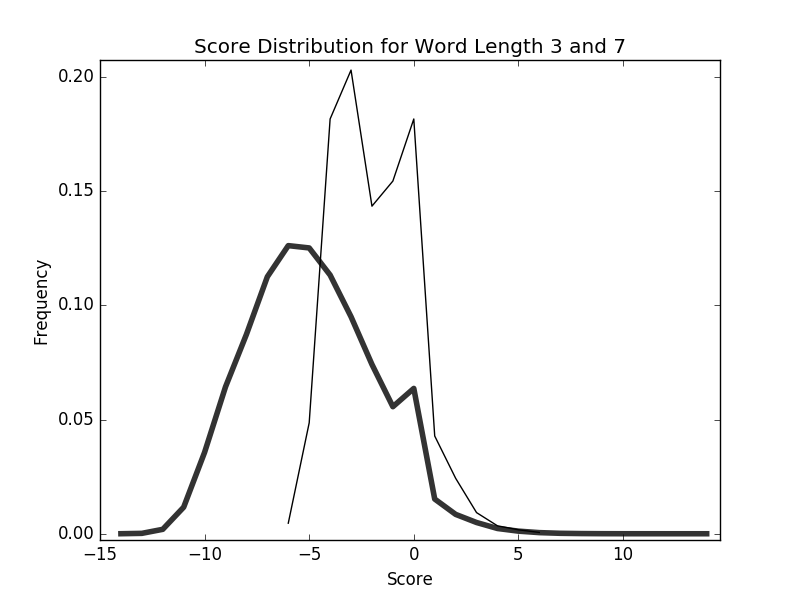
\includegraphics[width=0.60\textwidth]{score-dist}
\label{figure:score_dist}
\end{center}
\end{figure}

\subsection{Implementation}

Our implementation of local search alignment with uncertainty has the following steps: (1) collect and expand all $w$-mers from the reference sequence, (2) for each $w$-mer in the query sequence, scan in the database for hits, (3) for each hit, run sequence alignment on the prefix and suffix of the query sequence to extend the hit, (4) return the alignment with the highest score. 

There exists a variety of variations for the extension phase in BLAST; one can terminate the processes when the score falls pass a score that was better for a shorter extension, restricting insertions and deletions. \cite{blast} In our implementation, we restrict the regions in the reference sequence to which extensions are more likely by the length of the prefix and suffix. This idea is motivated by the design of our experiment, which is more elaborated in the next section. In practice, this decision, although reduces the running time of the algorithm, can compromise the quality of the solution. Since our study focuses more on the two modifications and the parameters, $\delta_p$ and $\delta_s$, than on the best implementation of BLAST, we nonetheless allow such decision although, for practical use, we recommend to use the most optimal implementation for BLAST. 

When extending for the suffix of the query sequence, we perform the alignment between the reversed suffix and reverse of region in the reference sequence that we deem most likely to align with the suffix. We use Hirschberg's algorithm for the extension phase. This dynamic algorithm has the advantage of performing in linear space, i.e.: $O(nm)$ where $n$ and $m$ are the lengths of the input sequences \cite{global_align}. We modified the open source Python software wuzhigang05/Dynamic-Programming-Linear-Space to match the similarity measures in our method. This implementation is however a global alignment algorithm, which may seem unconventional as BLAST originally uses local alignment for its extension phase. \cite{blast} However, due to the restriction of the search region for the extensions which removes the possibility of adding unwanted trailing gaps, we considered global and local alignment to be interchangeable.

We allows certain simplification in the implementation, ignoring certain possibilities for optimization, without hindering the purpose of the experiment. One of such simplification applies on the size of the $w$-mers. As the optimal word size for constructing the database has been studied in other researches and may depend on the design of the indexing stage \cite{blast}, we will not focus on this issue in our study. Instead, we conduct all our experiments with $w=7$ and focus on developing a mean for choosing of the confidence and score thresholds generalizable to all word size. 

\section{Experiment}

We test our implementation by aligning randomized substrings of length $w_q$ selected randomly from the CHR22 sequence. Our sequence randomization algorithm randomly induces at least $d$ substitutions and $g$ insertions and deletions to an input sequence. We compare the location $l_h$ to which a hit was found to the location $l_o$ where the substring was originally retrieved and considered the algorithm to have performed accurately if the output alignment outscores the alignment at the original location or if the found alignment's location in the reference sequence lies close to where the query sequence was originally retrieved, i.e.: $|l_h - l_o| < w_q - w + g$. We consider output alignments that fail this condition ``suboptimal", and call query sequences with no hit found as ``no-hits".

This method allows us to obtain counts for the number of suboptimal alignments and of no-hits relative to the dissimilarity between the query sequence and the sequence where it originated from, which is defined by $w_q$, $d$ and $g$. 

\subsection{On the Indexing Confidence and Score Thresholds}

In this experiment, we study on the effect in the choice of the confidence and score thresholds, $\delta_p$ and $\delta_s$ respectively, for the indexing stage. In particular, we experiment on $\delta_p \in \{0.7, 0.8, 0.9\} $ and $\delta_s \in \{-13, -12, ... , 13\}$. Note that for a hit size of $w = 7$, with the substitution matrix $M$ of our choice, the lowest and highest hit scores are -14 and 14 respectively and $\delta_s = 13$ is equivalent to $\delta_p = 0$. As our implementation is not fully optimized, we use the first 1000 nucleotides of CHR22 as the reference sequence for the benefit of time and space efficiency. As shown in Figure \ref{figure:conf_cum}, the cumulative distribution of the confidence values for this portion of the sequence is similar to the one for the entire sequence. Therefore, we assume that some of the results for this portion of the sequence can be generalized for the entire sequence.

For each $\delta_p$, we run the experiment with $d \in \{2, 4\}$, $g \in \{0, 2, 4\}$ and $w_q \in \{10, 13, 15\}$. For each parameter settings, we sample 1000 alignments using our sequence randomization algorithm. The same sample is used to test for each of the $\delta_s$.

\subsection{On Local Alignment Search}

In this experiment, we generate the database for our entire reference sequence with a particular confidence threshold, $\delta_p$, chosen using our previous experiment. We then test its performance by aligning randomized sequences using the same randomization technique as in the previous experiment with some selected $\delta_s$. Finally, we compare the result in both experiments. 

\section{Analysis}

We employ two measures to determine the performance of our method for a chosen set of threshold values: (1) the proportion of suboptimal alignments which can be detected when the output alignment resides far from the location where the query sequence comes from and scores lower than the alignment between the query sequence and its original form, and (2) the proportion of no-hits. 

\subsection{On the Indexing Confidence and Score Thresholds}

From the result obtained in the first experiment, we observed that the occurrence of suboptimal alignment and no-hits is invariant when $\delta_s$ is small. As the threshold surpasses a certain value, the occurrence of suboptimal alignments starts to decrease while the occurrence of no-hits beings to increase. For example, Figure \ref{figure:counts_10} shows the counts of suboptimal alignments and no-hits for $w_q = 10$ and $\delta_p = 0.9$. We can see the counts begin to shift around $\delta_s = 0$. We interpret this behaviour by the possibility that a significant portion of the low-scored $w$-mers lead to the suboptimal alignments, and are consequently excluded when $\delta_s$ becomes larger, causing no more hits found for the previously suboptimally aligned query sequences. This suggests that not expanding any $w$-mer, or choosing $\delta_p = 0$ or $\delta_s = 13$, may not be optimal. 

\begin{figure}[tbp]
\begin{center}
\caption{Counts of suboptimal alignment and no-hits when $w_q = 10$ and $\delta_p=0.9$ for each $d \in \{2, 4\}$, $g \in \{0, 2, 4\}$ and  minimum hit score $\delta_s \in \{-13, -12, ... , 13\}$ using the first 1000 nucleotides in CHR22 as the reference sequence.}
  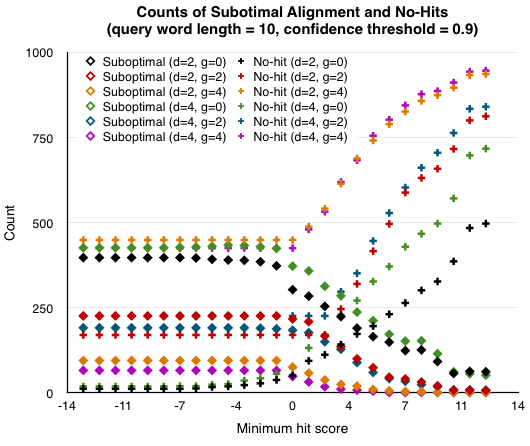
\includegraphics[width=0.60\textwidth]{counts-10}
  \label{figure:counts_10}
\end{center}
\end{figure}

An alternative way to analyze the proportion of suboptimal alignments and no-hits is to examine the percentage accuracy and hits which we define as the following.

\begin{equation}
\%\mbox{acc} = 1 - \mbox{SUBOPTs}/(N - \mbox{NOHITs})
\end{equation}

\begin{equation}
\%\mbox{hits} = 1 - \mbox{NOHITs}/N
\end{equation}
SUBOPTs and NOHITs are the counts for suboptimal alignments and no-hits respectively, and $N$ is the number of samples. 

\begin{figure}[tbp]
\begin{center}
\caption{Correlation between \%acc and \%hit, and between the later two and the $\delta_s$ for each $\delta_p$. The 6 plots combine all results of the experiment using the first 1000 nucleotides in CHR22 as the reference sequence.}
  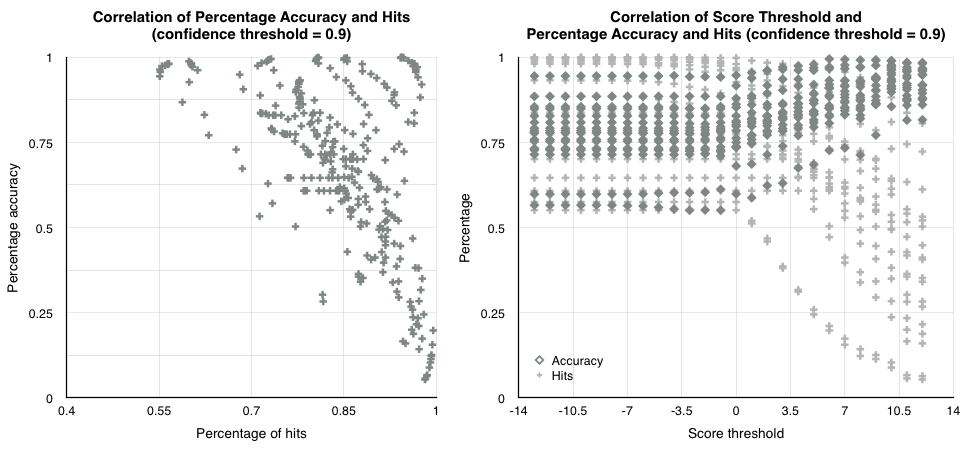
\includegraphics[width=0.99\textwidth]{09}
   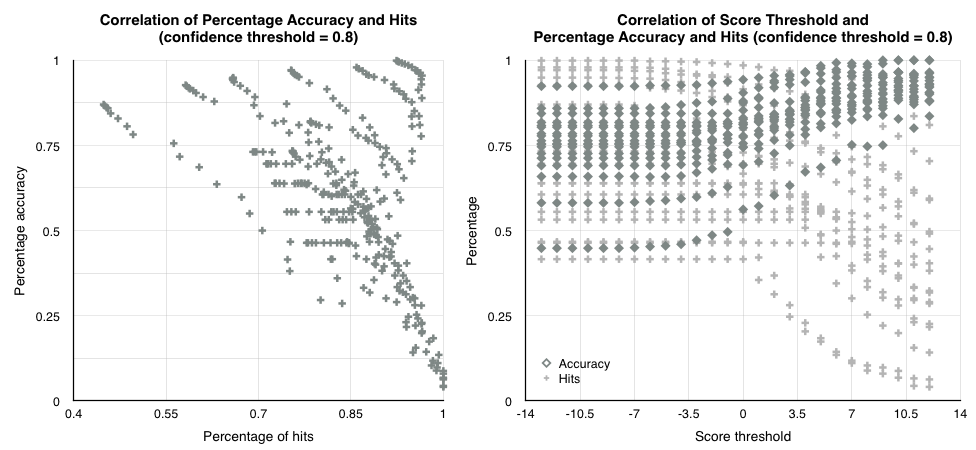
\includegraphics[width=0.99\textwidth]{08}
   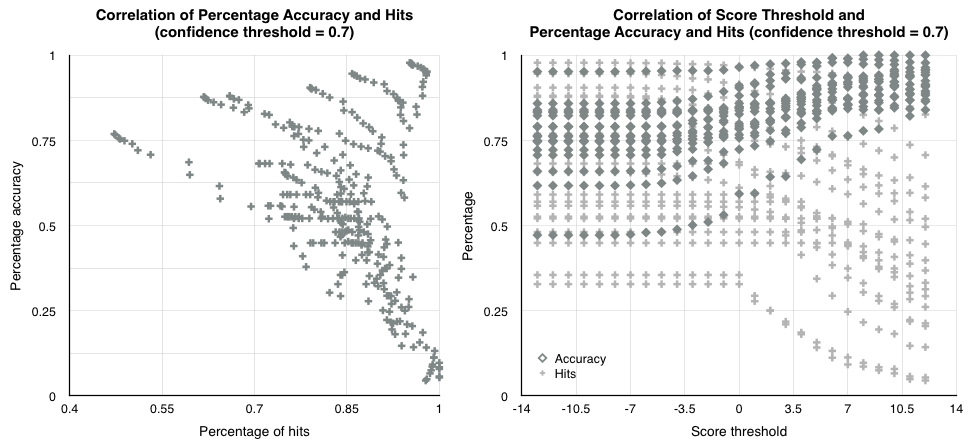
\includegraphics[width=0.99\textwidth]{07}
\label{figure:big_page}
\end{center}
\end{figure}

Figure \ref{figure:big_page} plots the correlation between percentage accuracy and hits for each chosen $\delta_p$ and their correlation with $\delta_s$. These plots combine all results obtain for each $d \in \{2, 4\}$, $g \in \{0, 2, 4\}$ and $w_q \in \{10, 13, 15\}$. The relationship between $\delta_p$, $\delta_s$ and the performance of our method may appear unclear as we observe that there exists some samples that resulted a high percentage ($\ge$ 0.85) for both accuracy and hits for any chosen $\delta_p$, and the choice of $\delta_p$ has seemingly no imminent effect on the variation between $\delta_s$ and the frequency of suboptimal alignment and no-hits. However, the dissimilarity between the query sequence and its original form may have non-negligible correlation with the accuracy and hits. Hence, we construct box plots to examine the existence of such correlation. Figure \ref{figure:box_plots} shows the variability in the percentage accuracy and hits according to the different settings for $w_q$,  $d$ and $g$  in the randomization algorithm, and $\delta_p$. We found that the occurrence of suboptimal alignments and no-hits may indeed increase with the number of substitutions and gaps added to the query sequence. Notably, when $d$ and $g$ increases, the percentage of hits decreases dramatically, especially when increasing the number of insertions and deletions. We also observe that increasing the query sequence length $w_q$ can increase the percentage of hits. This can be interpreted this as a cause of the small length of query sequence, $w_q$, relative to the length of the database indices, $w$; an insertion or deletion can potentially destroy a location in the query sequence that would originally lead to a hit. This supports the experimental results of BLAST which states that choosing a relatively small $w$ compared to $w_q$, decreases the percentage of no-hits. \cite{blast} 

\begin{figure}[tbp]
\begin{center}
\caption{Variation of \%acc and \%hit according to $w_q$, the dissimilarity of the query sequence ($d$, $g$) and $\delta_p$.}
   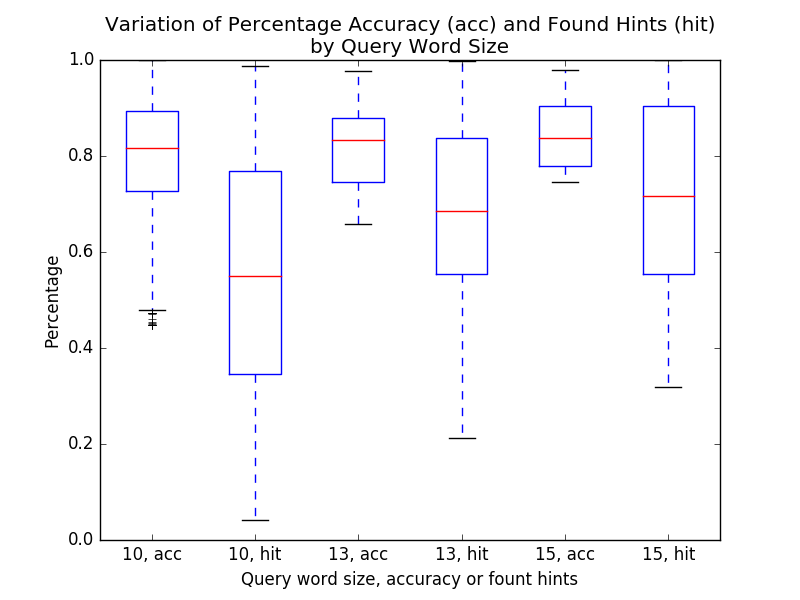
\includegraphics[width=0.49\textwidth]{size}
   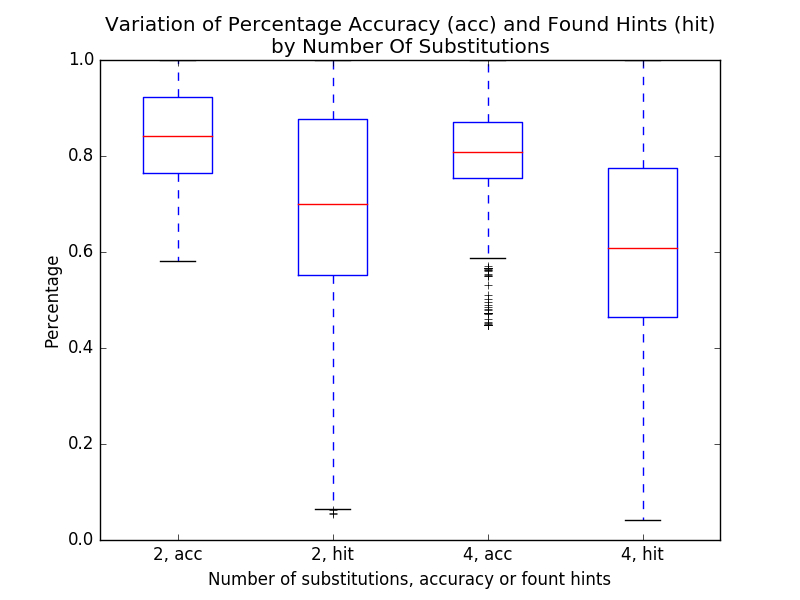
\includegraphics[width=0.49\textwidth]{diff}
   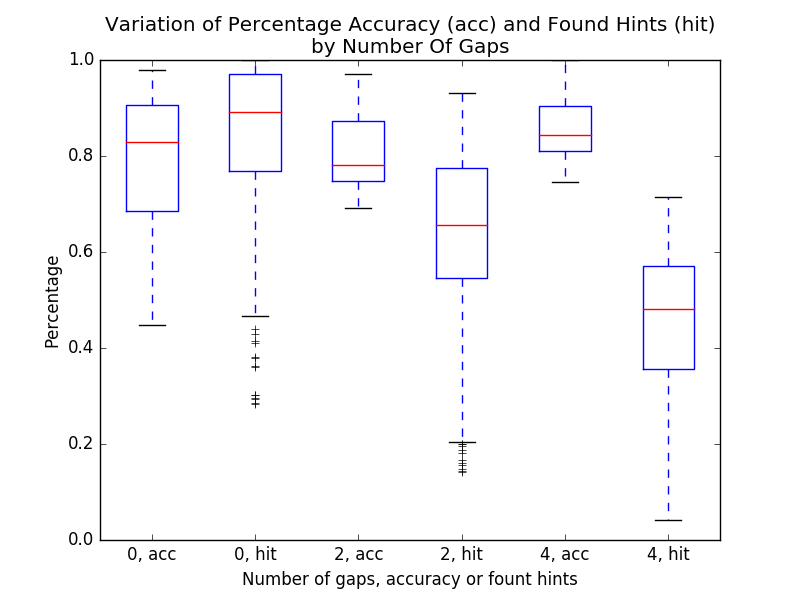
\includegraphics[width=0.49\textwidth]{gap}
   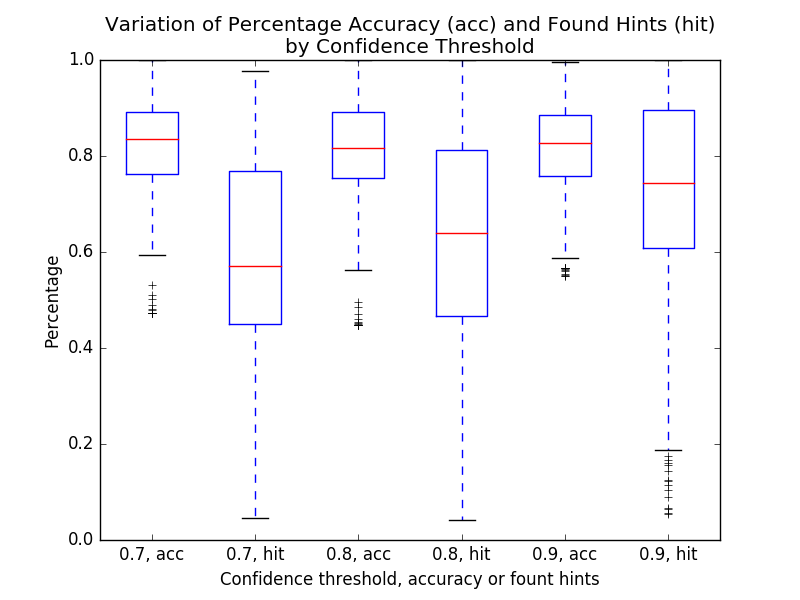
\includegraphics[width=0.49\textwidth]{conf}
\label{figure:box_plots}
\end{center}
\end{figure}

Perhaps, one of the most crucial observations resides in the box plot concerning the confidence threshold (see Figure \ref{figure:box_plots}). The percentage accuracy appears to stay invariant for each chosen $\delta_p$. If the proportion of no-hits can be controlled by choosing the appropriate $w$, we can potentially chose any $\delta_p$ that optimizes the database indexing efficiency without compromising the performance of the method. Indeed, Figure \ref{figure:small_page} rearrange the result according to the query sequence length. We observe strong correlation between the $w_q$, \%acc and \%hits. In particular, when $w_q$ is larger, \%acc and \%hits can reach higher and can vary less when $\delta_s$ changes. We also notice that the high values of \%acc and \%hits for $w_q=15$ is distributed across all \%acc and \%hits correlation plots of Figure \ref{figure:big_page}. 

\begin{figure}[tbp]
\begin{center}
\caption{Correlation between \%acc and \%hit, and between the later two and the $\delta_s$ for each $w_q \in \{10, 15\}$.}
  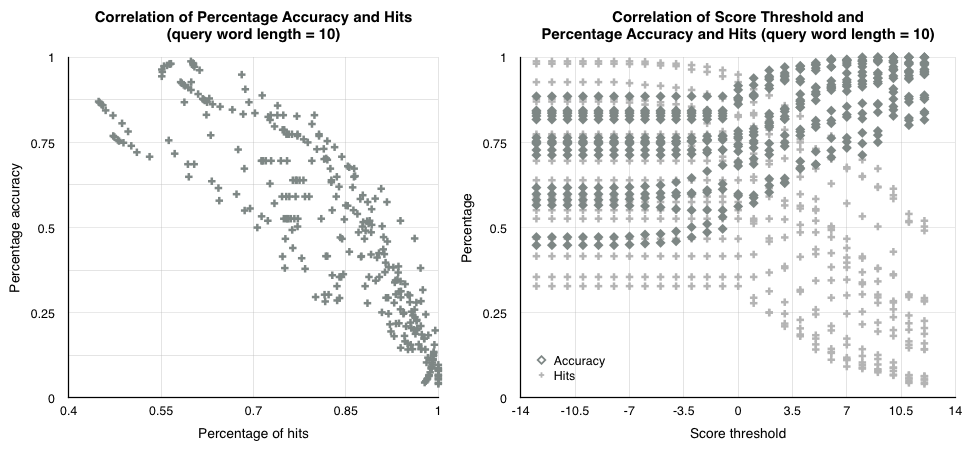
\includegraphics[width=0.99\textwidth]{10}
   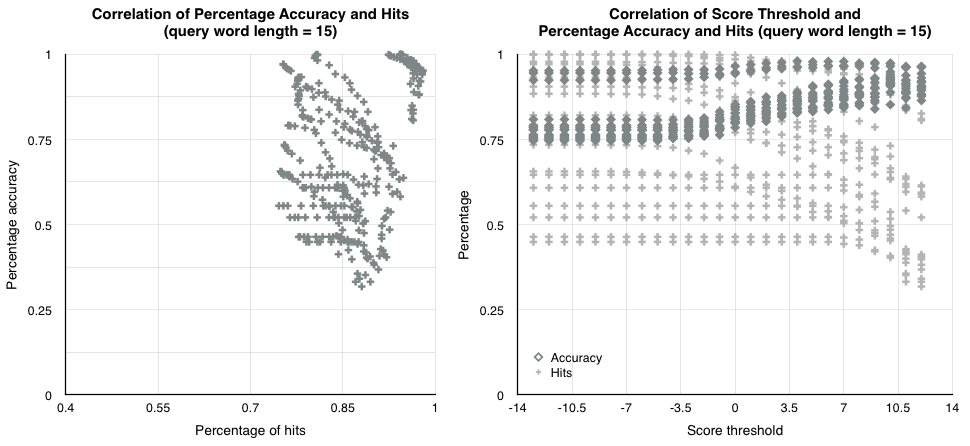
\includegraphics[width=0.99\textwidth]{15}
\label{figure:small_page}
\end{center}
\end{figure}

Our analysis suggests that the nature of the query sequence ($d$ and $g$) and $w$ have more effect on the performance of the method. One may argue that the correlation plots as in Figure \ref{figure:big_page} can be a reliable procedure for choosing the value for the two thresholds, and that $\delta_p = 0.7$ and any $\delta_s \in [-3, 3]$ appear to be reasonable choices for the first 1000 nucleotides of CHR22. Perhaps, one can also choose $\delta_s$ with the most statistical significance that bisects the value space between where \%acc and \%hits vary and do not vary. Yet, do to the small size of our sample, it may be early to determine whether the exact choice of the two thresholds ($\delta_p$ and $\delta_s$) can be based on resource availability. Nonetheless, we can examine their impact on the memory complexity of the algorithm. We have already discussed about the time complexity of database indexing phase in the Method section. Figure \ref{figure:hit_freq} shows the observed w-mers score distribution for different $\delta_p$. We note that it follows closely to the distribution in Figure \ref{figure:score_dist} for $w=7$ and that the $\delta_p$ acts like a rescaling factor of the score distribution. Upon examining the counts, we see that $w$-mers with high scores ($\ge$ 11) are always in the database and the counts for those high scoring $w$-mers are the same for all chosen $\delta_p$. Overall, the number of $w$-mers decreases by more than a half when changing $\delta_p$ from 0.9 to 0.7. Thus, we can use $\delta_p$ and $\delta_s$ to efficiently resize the database according to the memory availability and consequently, change the average number of locations in the reference sequence we need to iterate for each hit during the extension phase. 

\begin{figure}[tbp]
\begin{center}
\caption{}
  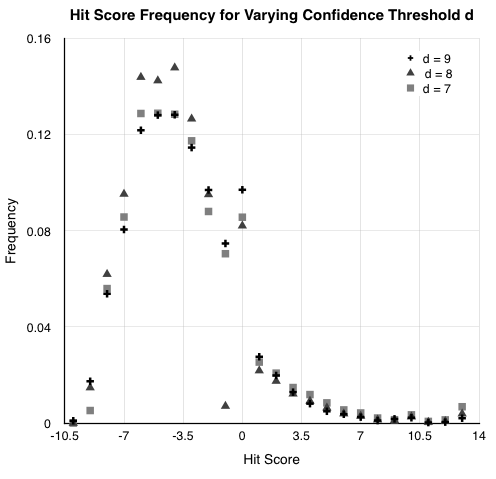
\includegraphics[width=0.99\textwidth]{hit-score-freq-1000}
\label{figure:hit_freq}
\end{center}
\end{figure}

\subsection{On Local Alignment Search}

Based on our previous analysis, we chose $\delta_p = 0.7$ and $\delta_s \in \{0, 3, 6, 9, 13\}$. We keep $d \in \{2, 4\}$, $g \in \{0, 2, 4\}$, $w_q \in \{10, 13, 15\}$ and $w=7$. Our implementation takes 33 minutes to build the database for all the 604,466 nucleotides of our reference sequence, and 2.44 days to run the experiment. Figure \ref{figure:true_result} shows the results. We observe, similar to our previous experiment's result, that the occurrence of suboptimal alignment and no-hits is high when the dissimilarity between the query sequences and their original form is large, and that \%acc and \%hits start to change when $\delta_s$ reaches a certain value. The later may appear much higher than what we have observed in the previous experiment, which is between 9 and 13. As we only sampled with positive $\delta_s$, one may argue that the value for which $\delta_s$ has the most statistical significance for separating where \%acc and \%hits vary and do not vary may be negative. However, it may be possible that \%acc and \%hits stay constant for all negative $\delta_s$ if we assume that the shape of the correlation graph between $\delta_s$, \%acc and \%hits should be same regardless of the reference sequence length, thus should resembles the correlation graph in Figure \ref{figure:big_page}.

We also observer an increase in \%acc and \%hits compared to the previous experiment (see Figure \ref{figure:true_result}). We interpret this as the increase in the chance for query sequence to match closely to a region in the reference sequence. $w_q$ is much smaller compared to 604,466 than to 1000 nucleotides. Any alternated substring of size 10 to 15 originated from the reference sequence has a higher chance of matching exactly another region in the reference sequence. Thus, this increase in \%acc and \%hits should not be regarded as an effect from the choice of $\delta_s$ and $\delta_p$. 

Concerning the complexity, we found that the mean number of locations in the reference sequence we need to iterate for each hit during the extension phase is 523.4 with standard deviation 305.2. The total number of location entries in the database is 8.57 millions, which is 14 times more than the length of the reference sequence. In the previous experiment, the mean and standard deviation never pass 21 and 4 respectively. Perhaps, for long reference sequences, we can raise $\delta_s$ even higher to reduce more cost in time and memory.

\begin{figure}[tbp]
\begin{center}
\caption{}
  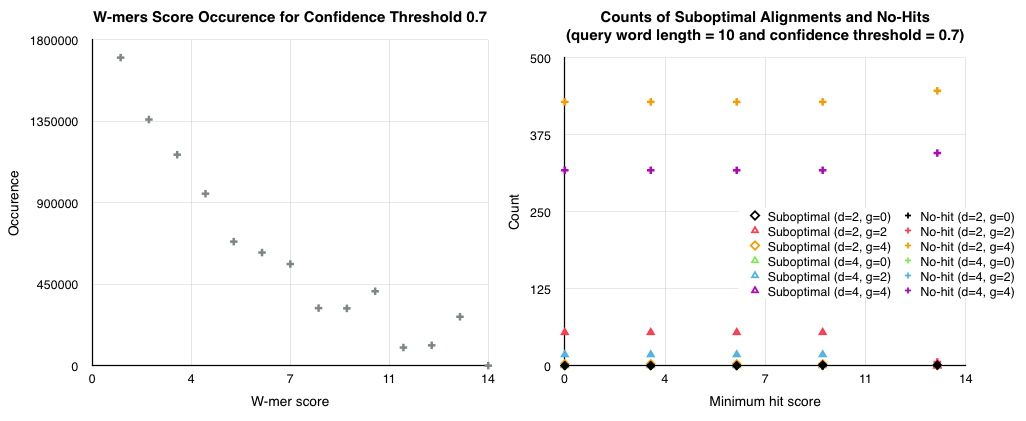
\includegraphics[width=0.99\textwidth]{true-10}
  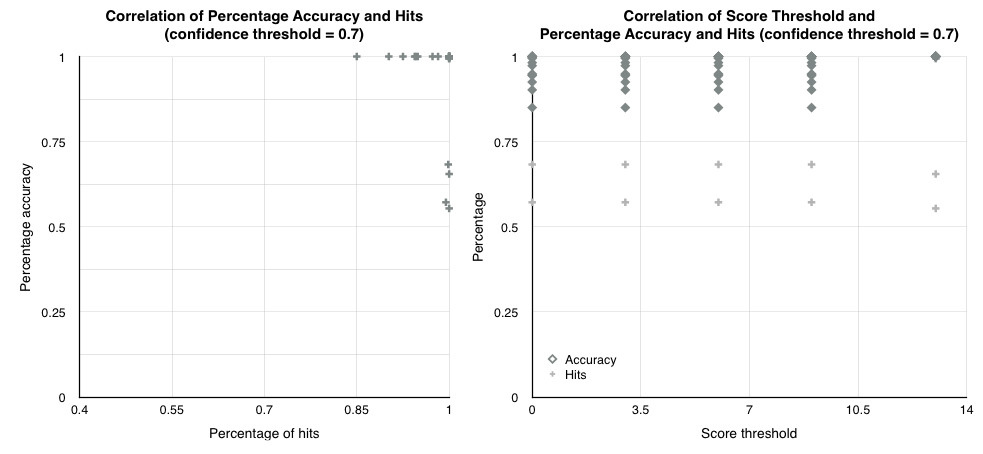
\includegraphics[width=0.99\textwidth]{true-07}
\label{figure:true_result}
\end{center}
\end{figure}

\section{Conclusion}

Uncertainty in biological sequence data, when considered during sequence alignment, can give more trueful results. We attempted to adapt Basic Local Alignment Search Tool (BLAST) to reference sequences with uncertainty by modifying the similarity measure and adding a new feature to its database indexing procedure. To handle complexity issues, we introduced two parameters: the confidence and score thresholds. Aside from the complexity, our experiments showed these two parameters are unlikely to have strong correlation with the performance of our method. The main factor that influences the accuracy and the proportion of no-hits was found to be the length of the high-scoring $w$-mers. However, these two thresholds should still be chosen with care, perhaps with a significance test or through the mentioned theoretical results, as they can strongly affect the time and space requirements. Future study can test more on the method with an optimized version of BLAST and longer query sequence length. 

\begin{thebibliography}{9}

\bibitem{blast}
	Altschu, Stephen F. et al
	\emph{Basic Local Alignment Search Tool.}
	J. Mol. Biol. (1990) 215, 403-410.
	
\bibitem{sequencers}
	Glenn, Travis C. 
	\emph{Field guide to next-generation DNA sequencers.}
	Mol Ecol Resour. (2011) 11, 759–769.

\bibitem{parsimony}
	Hanson-Smith, V., Kolaczkowski, B. \& Thornton, J. W. 
	\emph{Robustness of ancestral sequence reconstruction to phylogenetic uncertainty.}
	Mol. Biol. Evol. (2010) 27, 1988–1999.
	
\bibitem{global_align}
  Wu, Zhigang,
  \emph{wuzhigang05/Dynamic-Programming-Linear-Space}
  Github Repository. (2013)
  https://github.com/wuzhigang05/Dynamic-Programming-Linear-Space

\end{thebibliography}
%\end{multicols}
\end{document}